%
% Example from:
% http://tex.stackexchange.com/questions/17143/how-do-i-get-korean-hangul-characters-to-typeset-in-latex
%
\documentclass[10pt, A4]{article}
\usepackage[T1]{fontenc}
\usepackage{CJKutf8}
\usepackage[english]{babel}
\usepackage[utf8]{inputenc}

\usepackage{amsmath}
\usepackage{amssymb}
\usepackage{graphicx}
\graphicspath{ {./images/} }
 
\begin{CJK}{UTF8}{mj}

\title{Semi-Lagrangian과 PIC 방법을 사용한 그리드 기반 유체 시뮬레이션의 구현과 비교}
\author{장필식}
\date{2018. 12. 27}

\begin{document}

\maketitle

\begin{abstract}
\end{abstract}

\newpage

\tableofcontents

\newpage

\section{Introduction}

컴퓨터 그래픽스에서의 유체 시뮬레이션은 크게 두 접근방법으로 나뉘는데, 유체를 파티클의 집합으로 보아 각 파티클의 위치를 직접 시뮬레이션하는 Lagrangian 접근법, 그리고 유체를 유속의 vector field로 보아 파티클들이J 주어진 위치에서 유체가 지나가는 속도를 시뮬레이션하는 Eulerian Simulation이 있다. Semi-Lagrangian Method와 PIC Method 모두 양쪽 접근법을 같이 쓰는데, 이 연구에서는 이 둘을 구현한 다음에 서로 비교하여 장단점에 대해 알아볼 것이다.

\section{Methods}

\subsection{Navier-Stokes Equation}

압축 불가능한 유체는 각 위치마다의 속도를 나타내는 vector field $\vec{u} : \mathbb{R}
^3 \rightarrow \mathbb{R}^3$ 나타낼 수 있는데, 다음과 같은 편미분방정식을 만족한다.

\begin{equation}
  \frac{\partial u}{\partial t} + \vec{u} \cdot \nabla{\vec{u}} + \frac{1}{\rho} \nabla{\vec{p}} &= \vec{g} + \nu \nabla \cdot \nabla \vec{u}
\end{equation}

\begin{equation}
  \nabla \cdot \vec{u} = 0
\end{equation}

이 때 (1)은 Momentum Equation이고, (2)는 Imcompressibility condition이라고 명칭한다. 

이 편미분방정식을 한 번에 풀기에는 어려워, splitting이라는 방법을 통해 여러 개의 스텝으로 나눠서 풀게 된다.
간략하게 설명하자면, $\dot q = f(q) + g(q)$와 같은 미분방정식을 생각하자.
이것을 한 번에 푼다면 forward Euler를 사용해 $q = q_0 + \Delta t (f(q_0) + g(q_0))$로 구할 수 있다.
Splitting 방법은 $\dot q^a = f(q^a)$를 forward Euler 방법으로 먼저 푼 다음, 이 결과값을 사용해 $\dot q^b = f(q^b)$의 결과를 구하는 테크닉이다. 즉 $q'_0 = q_0 + \Delta t f(q_0)$, $q = q'_0 + \Delta t g(q'_0)$의 연산을 차례대로 하는 것이다. \cite{fluid-sim-cg}

위의 테크닉을 사용해 편미분방정식 (1)을 다음과 같이 세 개의 식으로 분할할 수 있다.

\begin{equation}
  \frac{D\vec{q}}{Dt} = \frac{\partial \vec{q}}{\partial t} + \vec{q} \cdot \nabla \vec{q} = 0
\end{equation}
\begin{equation}
  \frac{\partial \vec{u}}{\partial t} = \vec{g}
\end{equation}
\begin{equation}
  \frac{\partial \vec{u}}{\partial t} + \frac{1}{\rho} \nabla p = 0
\end{equation}

이것을 가지고 최종적인 알고리즘을 만들어보자.
우리는 $\Delta t$의 시간간격을 가지고 $\vec{u}$를 불연속적으로 Integration을 수행할 것이다. 처음의 velocity field를 $\vec{u}^0$라고 하고, n번의 integration 수행 이후 (즉 $n \Delta t$의 시간 후)의 velocity field를 $\vec{u}^n$이라고 하자. (3), (5)의 편미분방정식을 푸는 함수를 \texttt{advect()}, \texttt{project()}라고 하면, $\vec{u}^n$에서부터 $\vec{u}^{n+1}$을 구하는 알고리즘은 다음과 같이 쓸 수 있다.

\begin{align}
  \vec{u}^A &= advect(\vec{u}^n, \Delta t) \\
  \vec{u}^B &= \vec{u}^A + g \Delta t \\
  \vec{u}^{n+1} &= project(\vec{u}^B)
\end{align}

참고로 Incompressibility Condition ($\nabla \cdot \vec{u} = 0$)을 만족하는 조건은 \texttt{project()} 함수에서 다루는데, 이것에 대해서는 \textbf{Pressure Solve} 섹션에서 다룰 것이다.

\subsection{MAC Grid}

전 섹션에선는 시간을 연속에서 불연속적으로 변환했으므로, 여기서는 공간을 불연속적으로 변환하는 방법에 대해 설명할 것이다. 위치 공간 ($\textbb{R}^3$)를 MAC Grid를 통해 불연속하게 쪼갤 것이다.

시뮬레이션을 수행하는 영역을 $(i, j) \in [0, M \Delta x] \times [0, N \Delta x]$이라고 하자. 일반적인 2D Grid로 이 영역의 velocity field를 표현한다면, $i = 0..(M-1)$, $j = 0..(N-1)$에 대하여,  $(i \Delta x, j \Delta x)$의 위치마다 x축의 속도 $u(i, j)$, y축의 속도 $v(i, j)$를 저장하면 된다. 즉 크기 $(M, N)$의 2차원 어레이 2개를 저장하고 있으면 될 것이다. MAC Grid는 여기서 약간의 변형을 가하는데, 위치 $((i-1/2) \Delta x, j \Delta x)$ 마다 속도 $u(i-1/2, j)$, , 위치 $(i \Delta x, (j-1/2) \Delta x)$마다 속도 $v(i,j-1/2)$가 서로 Staggered된 형태로 아래의 그림과 같이 배치가 된다.

\begin{figure}[h]
\centering
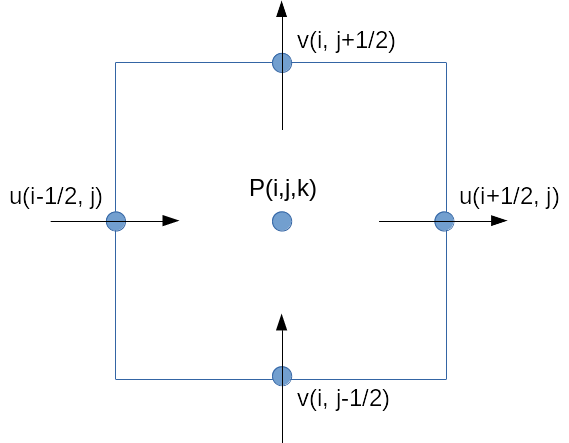
\includegraphics[width=0.5\textwidth]{mac_grid}
\caption{MAC Grid를 나태낸 그림}
\end{figure}

이젠 이것을 가지고 임의의 위치 $(x, y) \in \mathbb{R}^3$에서의 실제 속도값 $\vec{u}(x, y)$를 구할 수 있다. 예를 들어서 u에 대해서는 위치값이 1/2의 배수일 때 다음과 같이 구할 수 있다:

\begin{align*} 
  \vec{u}(i \Delta x, j \Delta x) &= (\frac{u(i-1/2, j) + u(i+1/2, j)}{2}, \frac{v(i,j+1/2) + v(i,j-1/2))}{2} \\
  \vec{u}((i+1/2) \Delta x, j \Delta x) &= (u(i,j), \frac{v(i,j-1/2) + v(i,j+1/2) + v(i+1,j-1/2) + v(i+1,j+1/2)}{4})
\end{align*}

임의의 위치에서의 Gradient 역시 쉽게 구할 수 있다:
\begin{align*}
  \vec{u}(i \Delta x, j \Delta x) &= (\frac{u(i+1/2, j) - u(i-1/2, j)}{\Delta x}, \frac{v(i,j+1/2) - v(i,j-1/2)}{\Delta x})
\end{align*}

위치값이 1/2의 배수로 떨어지지 않는 곳에서는 interpolation을 사용하여 값을 구할 수 있는데, 프로젝트에서는 bicubic interpolation을 사용한다.

\subsection{Semi-Lagrangian vs PIC method}

Advection과 Pressure Solve의 구현에 대해 알아보기 전에 일단 Semi-Lagrangian과 PIC Method의 차이점에 대해 알아보자.

만약에 Lagrangian 관점으로 Advection을 바라보면, i번째 particle의 현재 속력이 $\vec{v_i}$일때 위치 $\vec{x_i}$를 매 프레임마다 $\vec{x_i}(t + \Delta t) = \vec{x_i}(t) + \vec{v_i} \Delta t$로 integration을 해 주면 되므로 매우 간단하다. 하지만 현재로서는 속력에 대한 정보가 Grid에만 존재하므로 particle의 속력을 다른 방법을 사용해서 유추해야 한다. 그런데 시간 $t + \Delta t$에 어떠한 particle이 위치 $\vec{x}$를 지나갔다면, 그 particle은 시간 $t - \Delta t$에 위치 $\vec{x} - \vec{v} \Delta t$에 있었을 것이다. 즉 $\Delta t$의 시간 뒤 위치 $\vec{x}$에서 속도는 위치 $\vec{x} - \vec{v} \Delta t$에서의 속도값으로 근사할 수 있다. (실제 프로그램의 구현에서는 $\vec{x} - \Delta t$와 같은 Forward-Euler가 아니라 3차 Runge-Kutta Method를 사용한다.)

Semi-Lagrangian 방법에서 Advection - Gravity - Pressure Solve 과정이 모두 끝난 후에는, Grid의 각 셀 값들을 유체인지, 혹은 빈 공간인지 업데이트해야 한다. 이것을 여러가지 방법으로 수행할 수 있는데, 가장 간단한 방법은 현재 유체인 셀들이 일정한 밀도로 marker particle들을 생성하고, 이 particle를 Pressure Solve에서 구한 velocity field를 사용해서 한 timestep동안 advection을 수행한 다음, particle들이 차지하는 셀들을 유체 셀로 바꾸는 것이다. 더욱 정확한 방법으로는 현재 유체의 영역을 나타내는 Level Set 자체에 advection을 수행하는 것이다. 

PIC Method는 marker particle에 착안해서, 원래의 Advection Step을 grid 연산 대신 particle 연산으로 대체한다. 즉 Advection Step에 particle들을 이동시킨 다음, (TODO)

\subsection{Advection}

\subsection{Pressure Solve}

\textbf{MAC Grid} 섹션에서의 공식들을 사용해 (5)의 Pressure solve 공식을 다음과 같이 적용할 수 있다.

여기서 현재 유체의 상황을 반영하여 boundary condition을 주어야 하는데, 첫 번째는 비어있는 셀들에는 압력값이 0이라는 Dirichlet boundary condition이다 (특정 영역에 대해 가해지는 제한조건). 두 번째는 유체가 고체 벽을 통과하지 못한다는 것을 나타내는 Neumann boundary condition이다 (특정 면에 대해 가해지는 제한조건).

마지막 스텝인 Projection 스텝을 수행하기 위해서는 MICCG (Modified Incomplete Cholesky Conjugate Gradient) 방법을 사용한다. 이것은 선형 시스템을 푸는 대표적인 방법 중 하나인 Conjugate Gradient를 좀 더 빠르게 만든 것으로, Bridson의 책 \cite[p.79]{fluid-sim-cg}에 잘 설명되어 있다.

\subsection{Level Set Method}

Pressure Solve 과정을 수행하는 데 중요한 부분 중에 하나가 어떤 위치에 유체 안쪽 혹은 바깥쪽에 있는지를 판별하는 것이다. 가장 간단하게 이것을 해결하는 방법은 파티클이 걸쳐있는 셀들을 모두 유체로 마킹하고 그렇지 않은 것은 빈 공간으로 마킹하는 것이다. 하지만 이 방법은 파티클들의 수가 많지 않을 때 생기는 유체 내의 작은 기포 (빈 공간)를 매꾸지 못하여 유체의 내부에서 원하지 않는 유속이 생긴다는 문제가 있다. (이것에 대해서는 \textbf{Result} 섹션에서도 언급할 것이다.) 

그래서 우리는 Level Set Method를 통해 signed distance function을 구하는 방법을 사용할 것이다. Signed distance function은 특정 지점에서 가장 가까운 유체 파티클까지의 거리를 나타낸다 (이름에 signed가 붙은 이유는 유체 내부에서는 음수가 되기 때문이다). 만약 이 함수를 구할 수 있다면, 특정 위치가 유체 내부에 있는지 쉽게 판별할 수 있을 것이다. Level Set Method은 Grid로 Sampling하는 방식을 통해 (TODO)

\subsection{Implementation Details}

본 시뮬레이션은 C++로 구현하였으며, 여러 개의 코어에서 병렬화를 하기 위해 OpenMP를 사용하였다. (즉 OpenMP를 지원하는 컴파일러가 필요하다.) 프로그램 개발 환경은 Linux, 컴파일러는 Clang을 사용하였다. (코드는 https://github.com/lasagnaphil/fluid-sim에서 확인할 수 있다.) 개발에 사용된 라이브러리는 다음과 같다.

\begin{itemize}
  \item OpenGL (그래픽)
  \item SDL (창 생성/입출력 관련)
  \item IMGUI (UI 관련된 부분)
  \item MathFu (수학 라이브러리)
\end{itemize}

시뮬레이션의 성능을 높이기 위해서 여러가지 방법을 사용했는데, 일부 연산을 가속화시키기 위해 AVX/FMA SIMD intrinsics를 사용했다. (이것의 사용 유무를 CMake 빌드 세팅에서 \texttt{USE\_SIMD} 옵션으로 제어할 수 있다.) 예를 들어서, 연산에 많이 사용되는 함수 중 하나인 bicubic linear interpolation 함수, 그리고 pressure solve에서 자주 사용되는 벡터 간의 multiply-add 연산이 최적화 대상 중에 있었다.  그리고 OpenMP를 사용하여 유체 시뮬레이션 코드 중 병렬화가 편이한 부분 (loop index 사이에 dependency가 없는 for loop)을 여러 쓰레드에서 돌릴 수 있도록 했다.

사용자는 UI를 통해 중력값을 바꿀 수 있고, 시뮬레이션에 관련된 중요한 값들 (현재 시간, 평균 압력, 평균 속도, CFL) 등을 볼 수 있다. 그리고 좌클릭 드래그를 통해 유체의 한 지점의 속도를 바꿀 수 있고, 우클릭 드래그를 통해 시뮬레이션 전체의 중력을 바꿀 수 있다.

\section{Results}

3가지의 초기 상태 (물 particle의 초기 위치) 에 대해서 시뮬레이션을 수행해 보있다.

\begin{enumerate}
  \item 모자 모양으로 되어 있는 배열 형태.
  \item 물 전체가 한쪽으로 기울어져 있는 형태.
  \item 정육면체의 모양의 물 영역이 떨어지는 형태.
\end{enumerate}

각각의 초기 상태에 대한 스크린샷은 다음과 같다.

\begin{figure}[h]
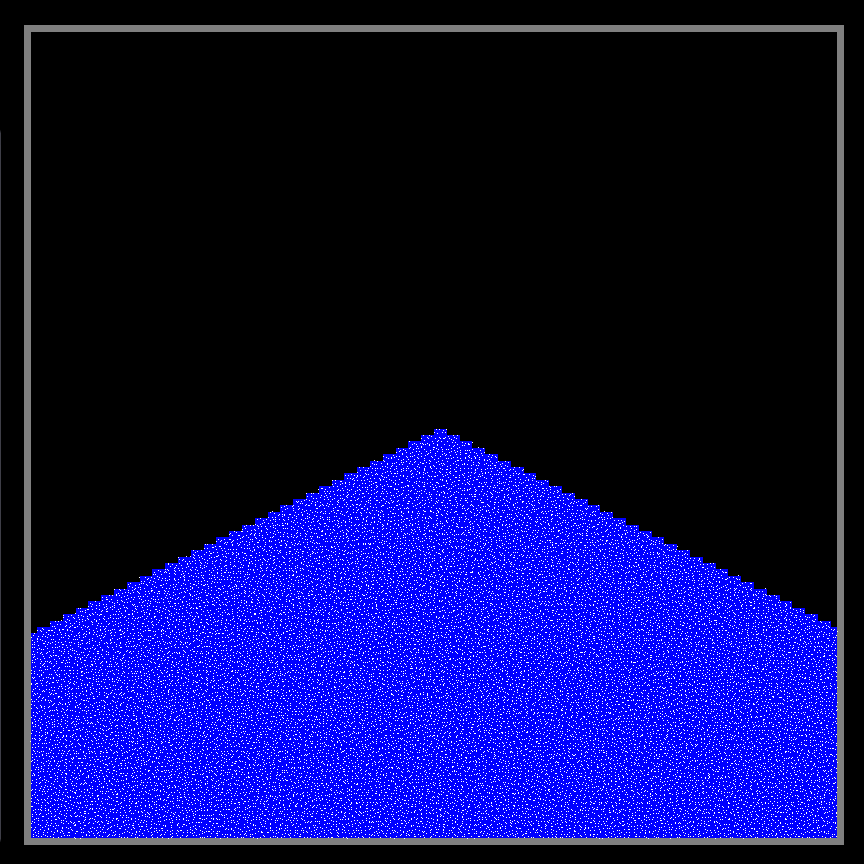
\includegraphics[width=0.32\textwidth]{init_state_1}
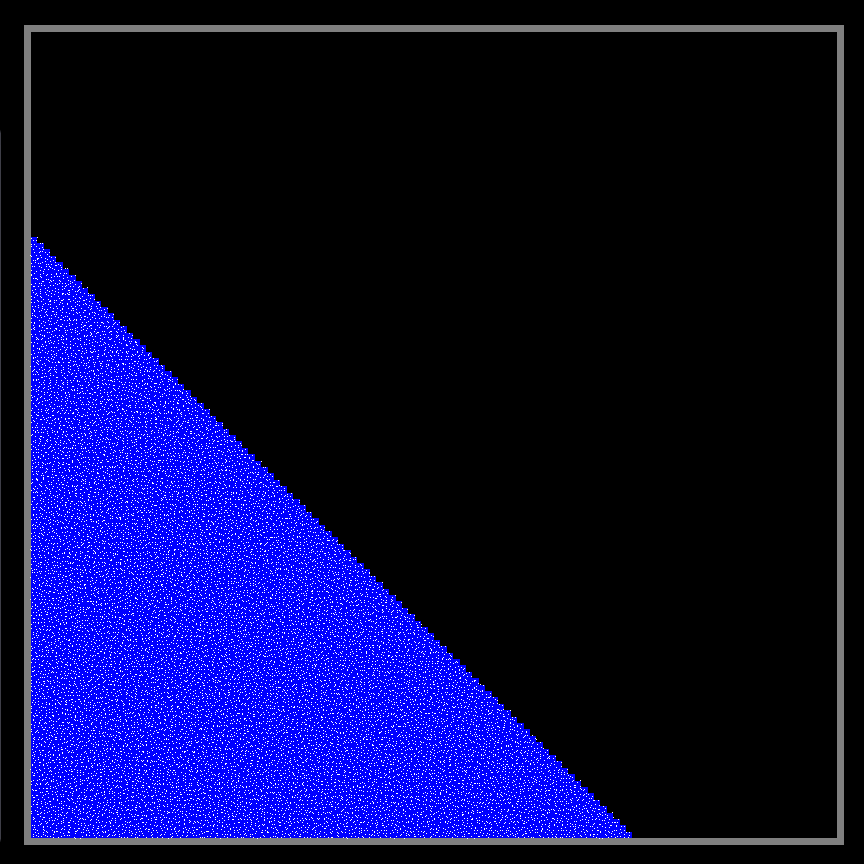
\includegraphics[width=0.32\textwidth]{init_state_2}
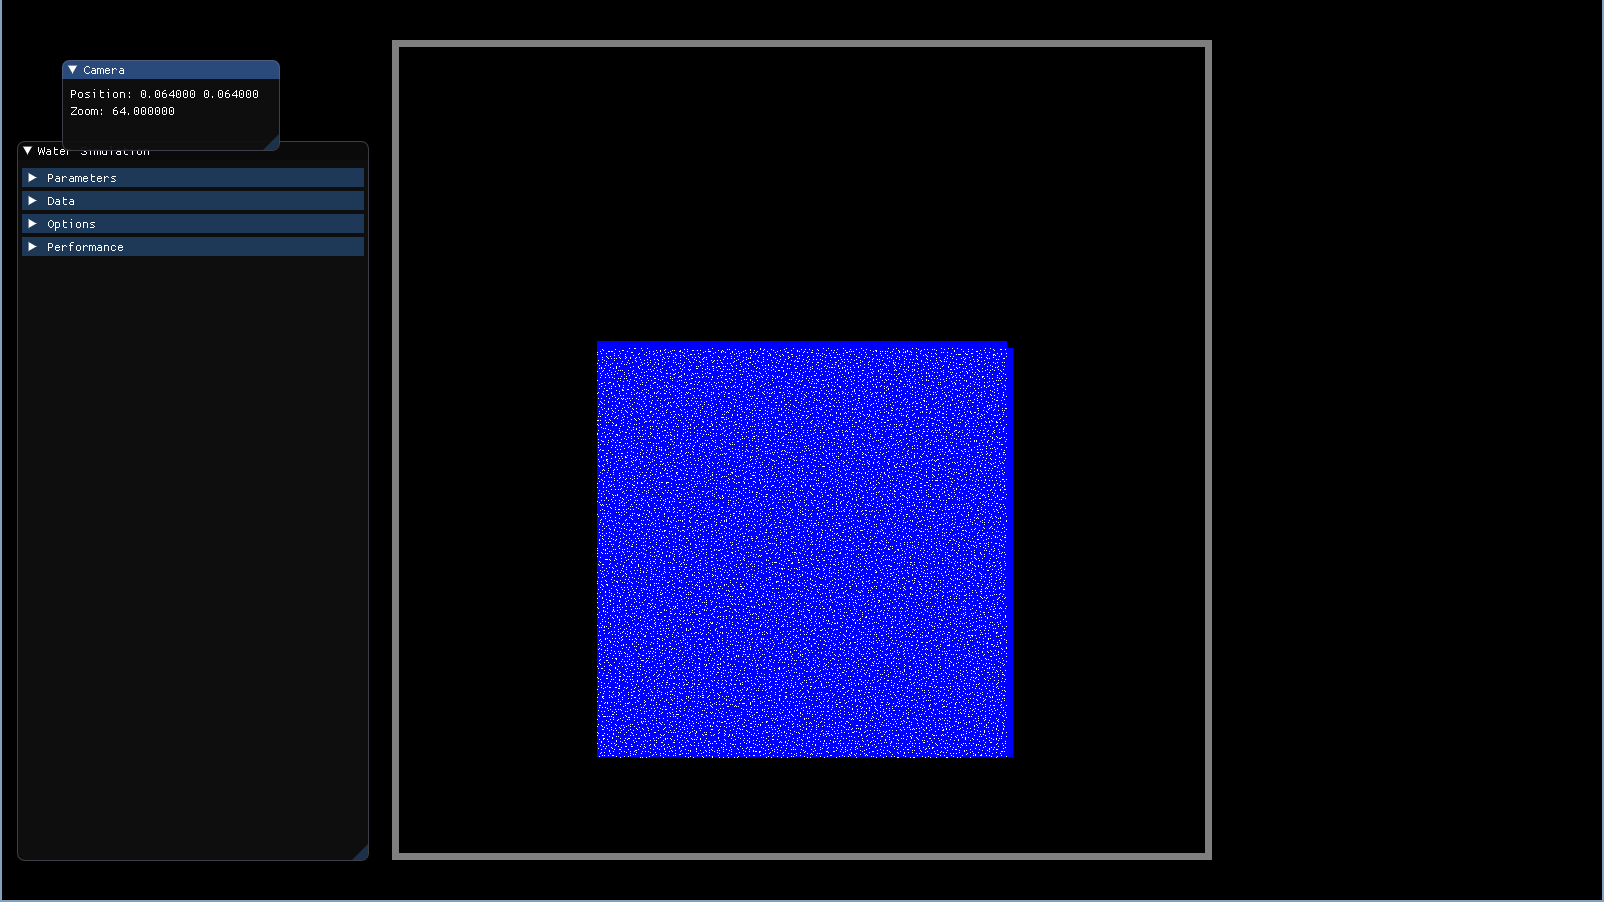
\includegraphics[width=0.32\textwidth]{init_state_3}
\end{figure}

물의 움직임에 대한 동영상은 따로 링크로 첨부한다. (링크)

좌우로 진동하는 가속도 (진폭 3$m/s^2$, 주기 1.0s)를 주었을 때의 물의 운동을 관찰해 보았다. (Grid Size는 128x128, $\Delta x = 0.001m$, $\Delta t = 0.005s$)

\subsection{Realism}

PIC 방법이 Semi-Lagrangian 방법에 비해 좀 더 생동감 있는 모습을 보였다.

(예시 스크린샷 첨부)

Volume preservation이 되는지 비교 $\rightarrow$ 둘 다 시간에 따라 부피 증가

(시간에 따른 부피 그래프 첨부)

\subsection{Stability}

Semi-Lagrangian이 좀 더 stable한 결과를 낼 수 있었다.

Stability의 예시: Semi-Lagrangian과 PIC를 같은 조건 (진동하는 가속도 진폭 X$m/s^2$, 주기 Xs) 에서 돌렸을 때 Semi-Lagrangian은 계속 구동했고 PIC는 Pressure Solve에서 터짐.
 
\subsection{Performance}

본 성능측정은 Intel(R) Core(TM) i5-4690 CPU (Quad core, 3.50Ghz)에서 진행했으며, 처음 30초 동안 프로그램을 돌렸을 때의 한 프레임 당 유체 시뮬레이션 코드가 걸린 전체 시간의 평균을 구한 것이다.

\begin{table}[h]
\centering
\begin{tabular}{|l|l|l|l|}
\hline
                & A & B & C \\ \hline
Semi-Lagrangian &   &   &   \\ \hline
PIC             &   &   &   \\ \hline
\end{tabular}
\caption{초기 상태 A, B, C에서 각각 Semi-Lagrangian과 PIC Method를 사용했을 때의 한 프레임당 시뮬레이션 연산 시간}
\end{table}

\section{Discussion}

\subsection{Explanation of Results}

TODO

- 현실성/안정성 차이에 대한 설명

- 성능 차이에 대한 설명

\subsection{Further Study}

현재의 유체 시뮬레이션에서 가장 시급하게 해결해야 하는 것이 있다면, Pressure Solver의 numerical stability를 개선하는 것이다. 파티클의 속도가 굉장히 높아지는 극단적인 경우에 Pressure Solver가 수렴을 하지 못해 올바른 해를 찾지 못하는 경우가 생겼으므로, 실제로 산업에서 활용할 만한 라이브러리로 만든다면 다양한 상황에 대해서도 무리 없이 돌아가도록 고쳐야 할 것이다. 이를 해결할 수 있는 방법 중 하나는 특정 파티클들의 속도가 너무 빨라지면 이것에 따라 해당되는 파티클의 timestep의 크기를 유동적으로 줄이는 것이다. \cite[p. 35]{fluid-sim-cg} 또 다른 해결 방안은 MICCG의 두 패러미터 값 $\tau$, $\sigma$를 조절해 보면서 더욱 좋은 수치를 찾는 것이다.

그리고 Semi-Lagrangian 방법에서 Particle의 밀도가 충분치 않을 때 부피가 줄어드는 현상을 관찰할 수 있었는데, 이것은 Kim et al. \cite{volume-preservation} 의 논문의 방법처럼 projection step에서 velocity field의 divergence를 0이 아닌 다른 값으로 보정해 해결할 수 있을 것이다.

PIC Method 특유의 점성은 FLIP Method라는 방식으로 해결할 수 있는데\cite{flip-fluids}, FLIP는 ... (TODO)

\section{Conclusion}

\begin{thebibliography}{9}
\bibitem{fluid-sim-cg}
Robert Bridson.
\textit{Fluid Simulation for Computer Graphics, Second Edition}. 
A K Peters/CRC Press, 2015.
 
\bibitem{fluid-engine-dev} 
Doyub Kim. 
\textit{Fluid Engine Development}.
A K Peters/CRC Press, 2017.

\bibitem{flip-fluids}
J.U.Brackbill, D.B.Kothe, H.M.Ruppel.
\textit{FLIP: A Low-dissipation, Particle-in-cell Method for Fluid Flow}.
Computer Physics Communications, Vol. 48, p. 25-38, 1988.

\bibitem{volume-preservation}
Kim, Byungmoon and Liu, Yingjie and Llamas, Ignacio and Jiao, Xiangmin and Rossignac, Jarek
\textit{Simulation of Bubbles in Foam with the Volume Control Method}
ACM Trans. Graph., 26.3, 2007

\end{thebibliography}

\end{CJK}

\end{document}
